
\chapter{Simulating degraded reads}\label{ap:sim-deg-reads}

In this appendix, we describe our approach for simulating reads based on constant expected degradation. We simulate reads for protein-coding isoforms and processed transcripts from GRCh38 annotation. The distribution of read counts follows a negative binomial distribution (see Appendix \ref{ap:count-dist}). To generate reads for an isoform of length $\mathrm{len}(j)$ given a degradation rate $d$, we first compute the maximum read length $\ell_\mathrm{max}=1/d$. The probability of generating a degraded read is $p_d=\min(\mathrm{len}(j)/\ell_\mathrm{max}, 1)$ and the probability of generating a full-length read is $1-p_d$. We now generate a read length with the following algorithm:
\begin{enumerate}
    \item Generate $U\sim \mathcal{U}(0,1)$.
    \item If $U<p_d$, generate degraded read length $\ell_i\sim \mathcal{U}_d(0,\min(\mathrm{len}(j),\ell_\mathrm{max})\cdot10^3)$.
    \item Otherwise, generate full read length $\ell_i=\mathrm{len}(j)$.
\end{enumerate}
Here, $\mathcal{U}$ and $\mathcal{U}_d$ are the continuous and discrete uniform distributions respectively. For constant degradation, the length of degraded reads are uniformly distributed over the integers from 0 to the length of the transcript isoform or the maximum read length, whichever is smaller. Once the read length $\ell_i$ is generated, we simply slice the transcript isoform sequence from the 3' end such that the resulting sequence is of length $\ell_i$. The reads simulated are thus perfect reads with 0\% error rate and no indels. We obtain a high fraction of reads ($>$99\%) mapped to the genome and transcriptome over simulated datasets with different degradation rates. 
% SLOW COMPILING
\begin{figure}[H]
    \centering
    \includegraphics[width=0.95\textwidth]{figures/app-b-1.png}
    \caption[Simulated reads with constant degradation aligning to the genome.]{Simulated reads with constant degradation aligning to the genomic locus of the gene PLEKHN1.}
\label{fig:app-b-1}
\end{figure}

\chapter{Generating novel isoform models}\label{ap:gen-novl-iso}

In this appendix, we describe our approach for generating novel gene isoform models. We first select a set of seed reference isoforms and introduce modifications that are well known to occur via alternative isoform regulation \textit{in vivo}. These modifications include the use of alternative 5' start sites, alternative 3' end sites, alternative splice donors and acceptors, exon skipping, intron retention, and the introduction of new exons and introns. In addition, we also introduce a new modification, termed \textit{subset} isoform, that drops exons from the reference isoform from the 5' end (Fig. \ref{fig:app-a-1}). Introduction of these novel subset isoforms increases the number of multi-mapping reads, making the process of assigning these reads to the correct isoform more complex. 
\begin{figure}[H]
    \centering
    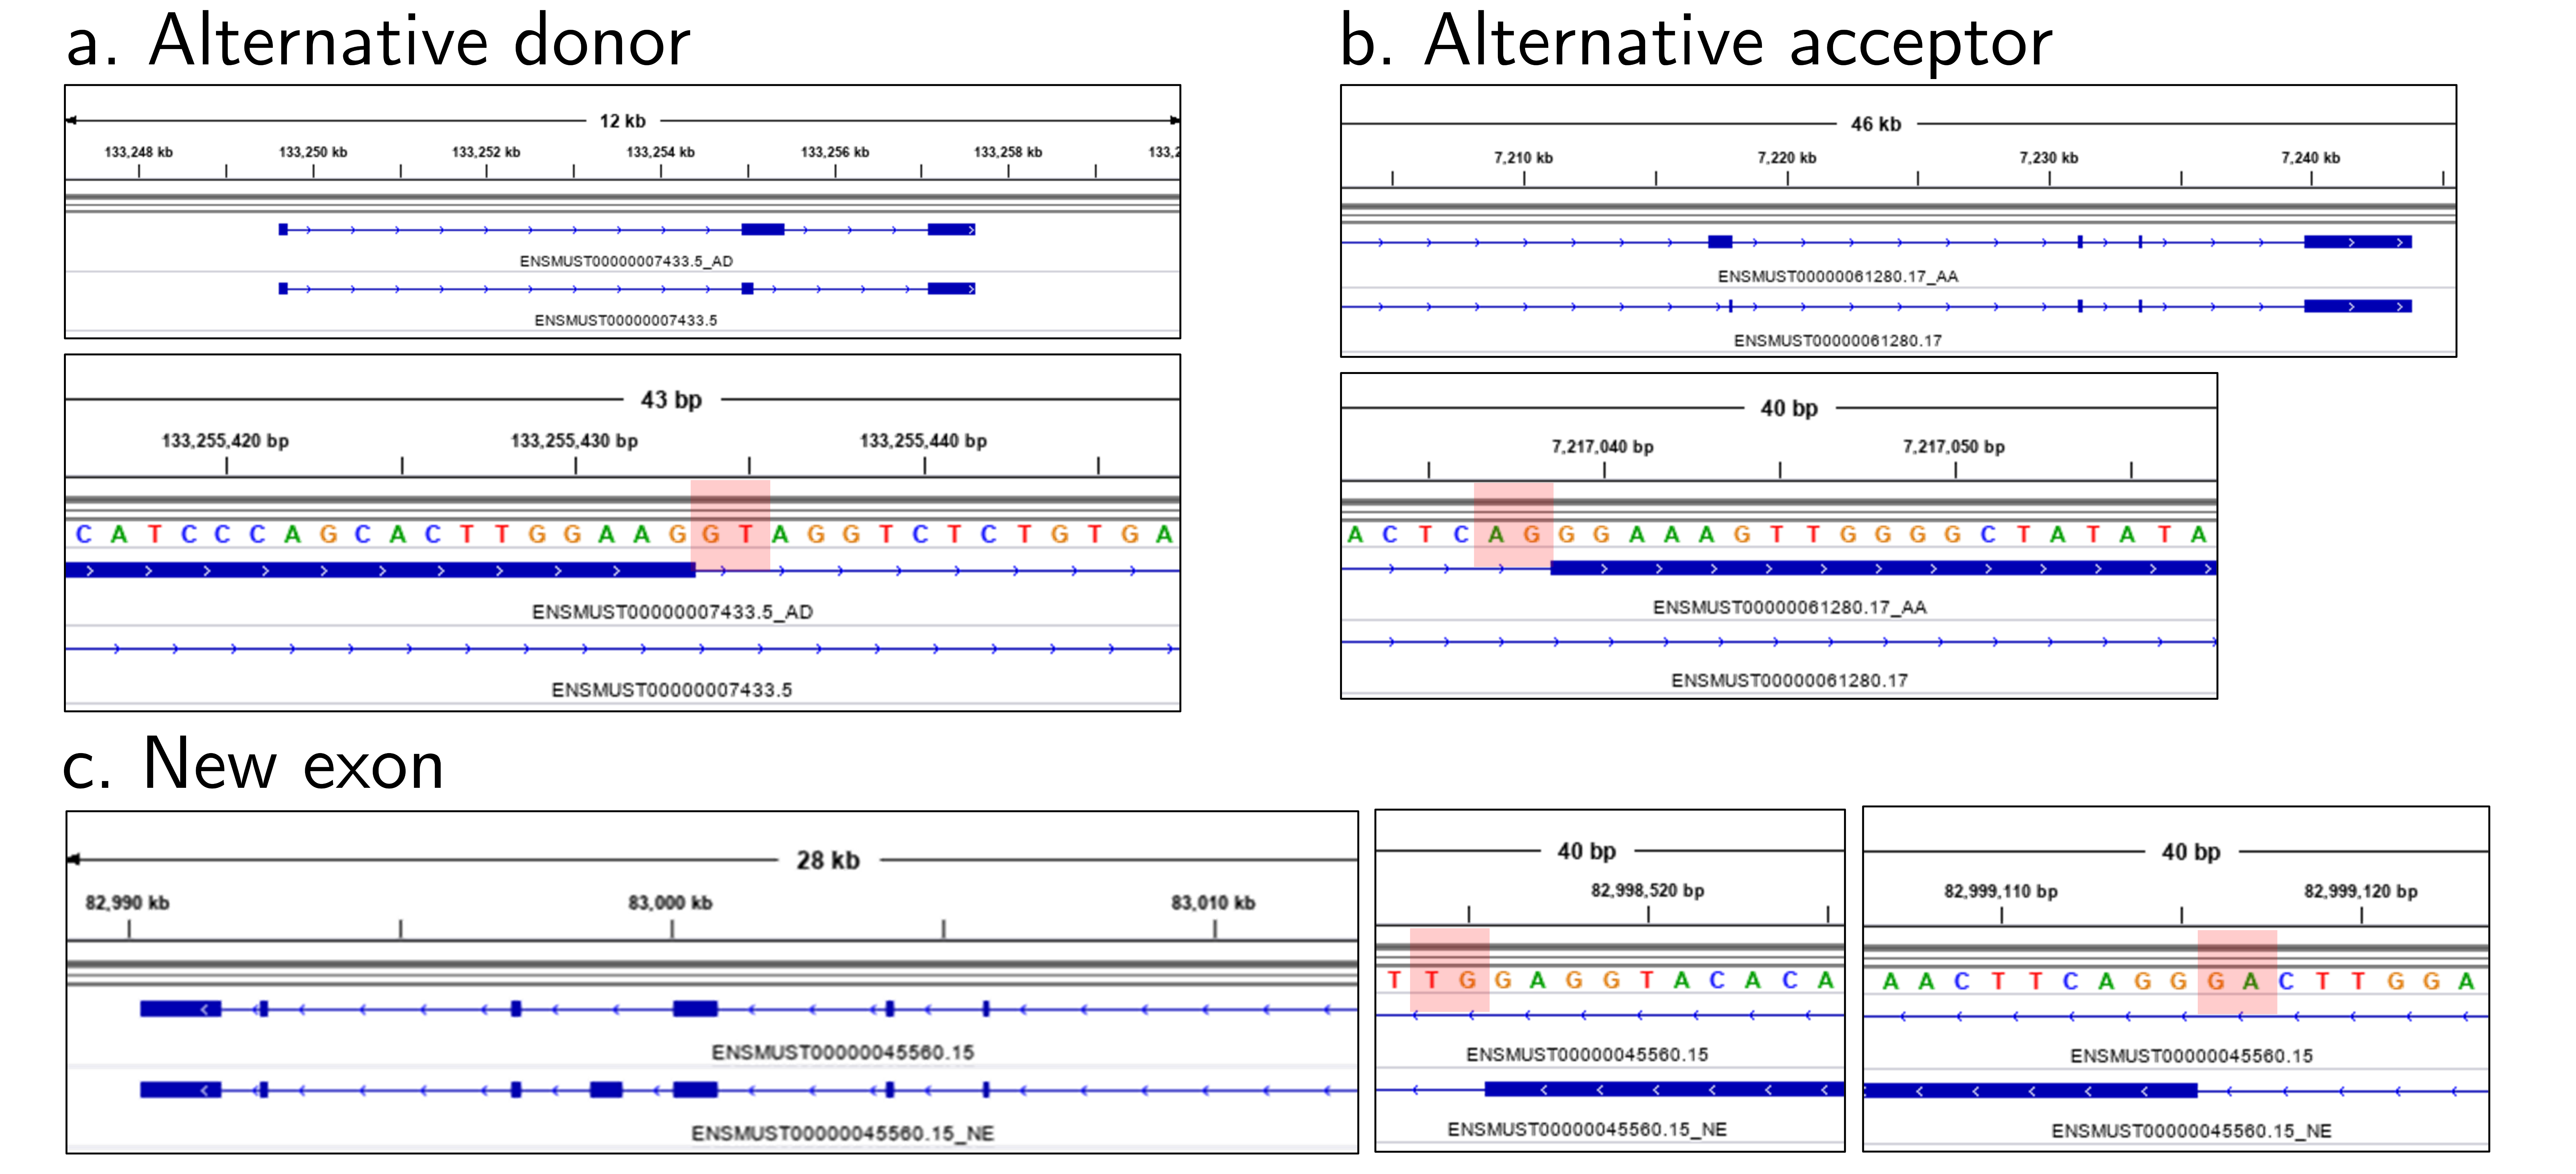
\includegraphics[width=\textwidth]{figures/app-a-1.png}
    \caption[Subset isoform modification]{Subset isoform modification. Exons from the 5' end of the reference isoform (blue) are removed to produce a truncated isoform comprising a subset of the exons of the original isoform.}
    \label{fig:app-a-1}
\end{figure}
Because some aligners (e.g. \texttt{minimap2}) use splice site signals to map reads, we ensure that novel isoform models conform to these splice site signals. We do so by performing splice site correction whenever necessary, i.e., for the alternative splice donor and acceptor, new exon and intron modifications (Fig. \ref{fig:app-a-2}). 
\begin{figure}[H]
    \centering
    \includegraphics[width=0.95\textwidth]{figures/app-a-2.png}
    \caption[Splice site correction for novel isoform models]{Splice site correction for novel isoform models for the GT-AG motif highlighted in red. Genomic sequence is reverse complemented where necessary.\textbf{a.} Alternative donor. \textbf{b.} Alternative acceptor. \textbf{c.} New exon.}
    \label{fig:app-a-2}
\end{figure}

\chapter{Count distribution analysis}\label{ap:count-dist}

To identify an appropriate distribution for simulating counts that best reflects real data, we ran NanoCount and Bambu on six direct RNA-seq samples obtained from sequencing of a human embryonic stem cell line (H9). Using the fitdistrplus R package (v1.1.6) \cite{Delignette-Muller2015}, we fitted discrete distributions (negative binomial and Poisson) to the counts returned by NanoCount and Bambu after filtering the counts in the top 0.001 quantile and analysed the skew and kurtosis of the fitted distribution. Since skewness and kurtosis are known not to be robust \cite{Delignette-Muller2015}, we also fit distributions to 100 bootstrap replicates. In all samples, the negative binomial provided a better fit compared to the Poisson distribution (Fig. \ref{fig:app-c}). This is unsurprising, as the negative binomial allows more flexible modeling of counts with an additional parameter that allows for greater variation, while the equal mean and variance assumption of the Poisson is somewhat restrictive. In fact, the negative binomial is equivalent to a mixture of Poisson distributions with the rate parameter distributed according to a gamma distribution. 
\begin{figure}[H]
    \centering
    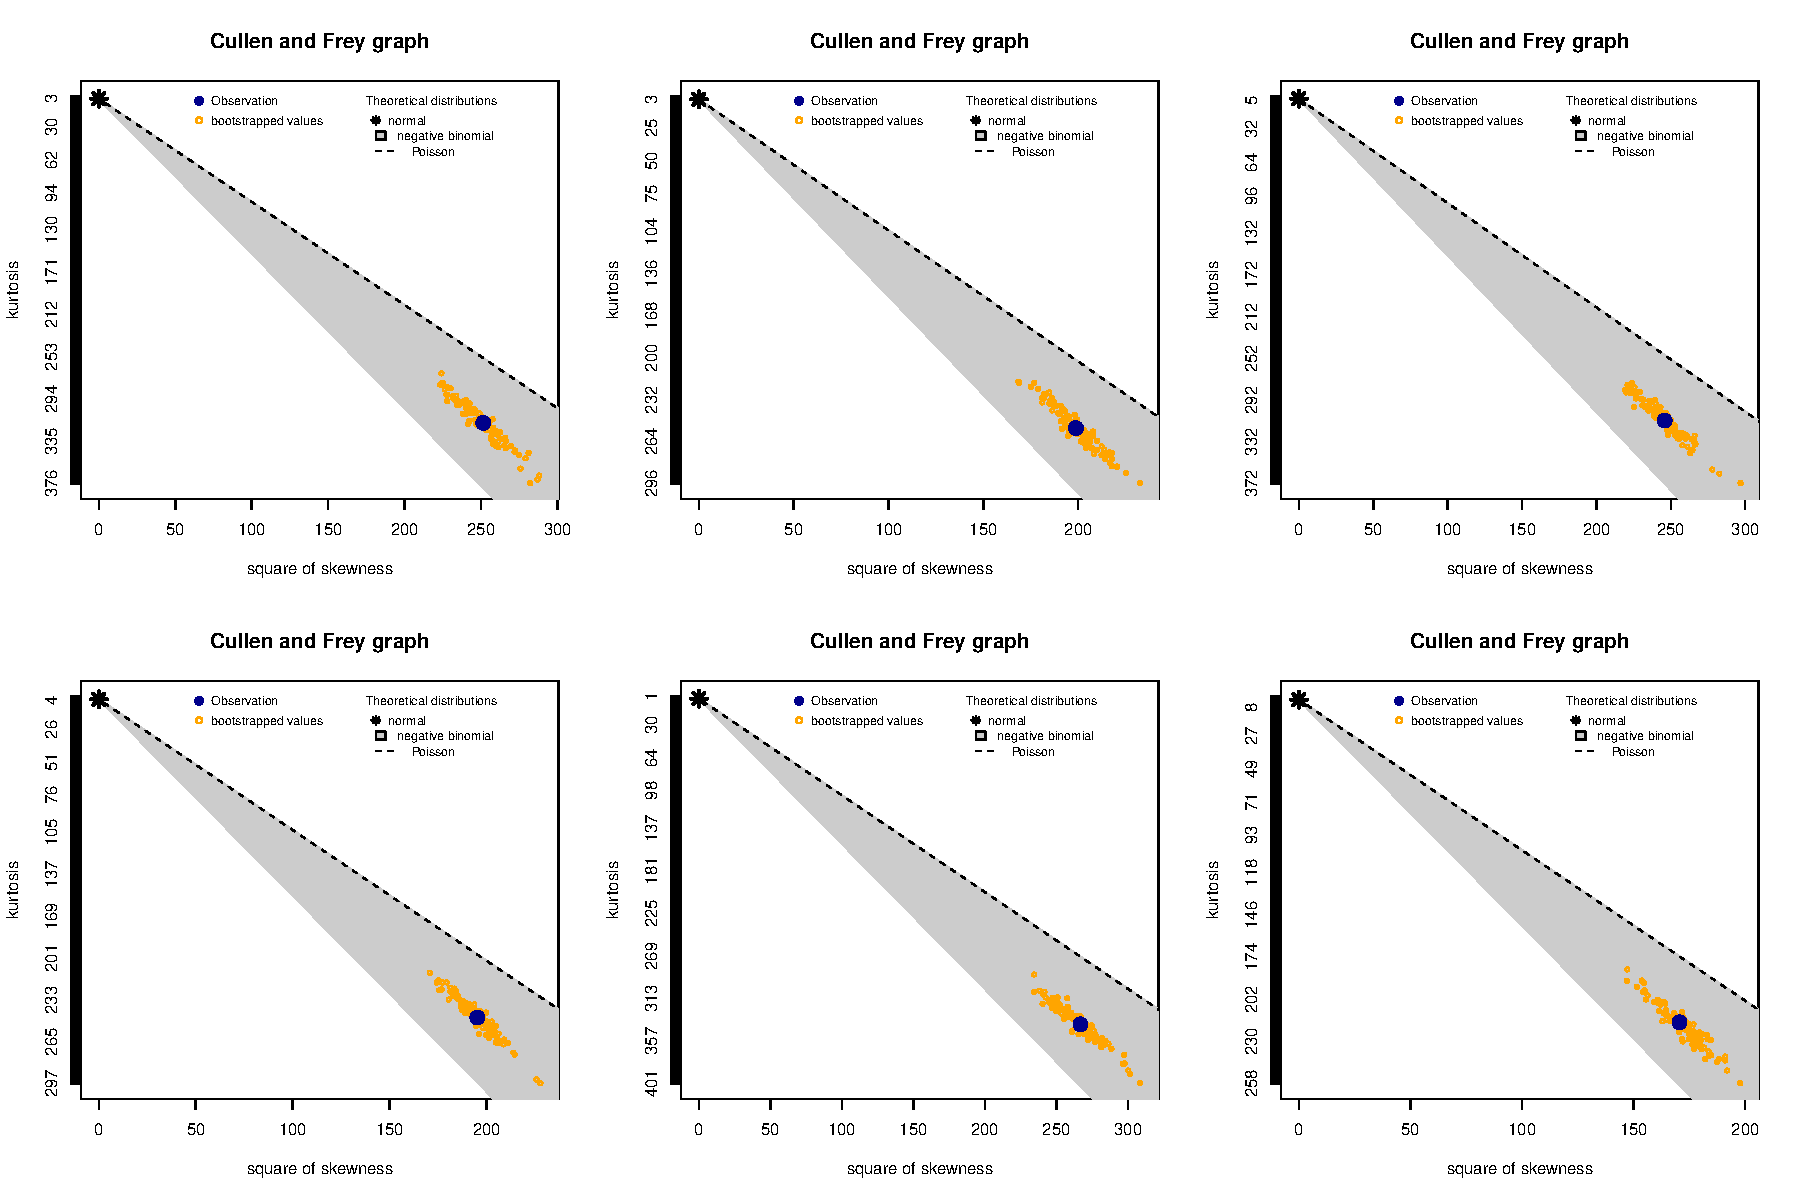
\includegraphics[width=0.9\textwidth]{figures/ap-c.pdf}
    \caption[Distributional analysis of RNA-seq counts]{Distributional analysis of RNA-seq counts returned by NanoCount (results for Bambu are similar). Each panel corresponds to one H9 sample, and each dot is a set of counts. Dark blue dots are real samples while bright orange dots are bootstrapped samples. The grey region indicates combinations of skew and kurtosis parameters for the negative binomial, while the dotted line indicates the same for the Poisson distribution. The real and bootstrap samples fall within the grey region and away from the dotted line implying that the negative binomial offers a better fit compared to the Poisson.}
    \label{fig:app-c}
\end{figure}

\chapter{Proof of concavity of log-likelihood function}\label{sec:proof-log-lik}

Here, we show that the log-likelihood function is concave. This implies that the local maximum corresponding to the maximum likelihood estimates $\hat{\bm\theta}$ returned by the EM algorithm is a global maximum. We follow the proof used in \cite{Jiang2009} and \cite{Libo2009}.  

Recall that the log-likelihood formulated in Section \ref{sec:likelihood-formulation} is given by
\begin{equation}
    \log p(\bm{R}\mid\bm{\theta}) = \sum_{i=1}^N \log \left[\sum_{j=1}^M \theta_j\cdot a_{ij}\cdot p(\ell_i\mid d_j, z_{ij}=1)\right]
\end{equation}
Since the sum of concave functions is also concave, we need only prove that each term in this sum is concave. Let the $i$\ts{th} term be
\begin{equation}
    f(\bm\theta) = \log \left[\sum_{j=1}^M \theta_j\cdot a_{ij}\cdot p(\ell_i\mid d_j, z_{ij}=1)\right]
\end{equation}
Let $\mathrm{\mathbf{H}}_f$ be the Hessian matrix for $f(\bm\theta)$. The $(x,y)$ entry of $\mathrm{\mathbf{H}}_f$ is 
\begin{equation}
    \begin{split}
        \left(\mathbf{H}_{f}\right)_{x, y} & =\frac{\partial^{2} f}{\partial \theta_{x} \partial \theta_{y}} \\
        & =\frac{\partial}{\partial \theta_{x}} \frac{\partial}{\partial \theta_{y}} \log \left[\sum_{j=1}^{M} \theta_{j} \cdot a_{i j} \cdot p\left(\ell_{i} \mid d_{j}, z_{i j}=1\right)\right] \\
        & =\frac{\partial}{\partial \theta_{x}} \frac{a_{i y} \cdot p\left(\ell_{i} \mid d_{y}, z_{i y}=1\right)}{\sum_{j} \theta_{j} \cdot a_{i j} \cdot p\left(\ell_{i} \mid d_{j}, z_{i j}=1\right)} \\
        & =-\frac{a_{i y} \cdot p\left(\ell_{i} \mid d_{y}, z_{i y}=1\right) \cdot a_{i x} \cdot p\left(\ell_{i} \mid d_{x}, z_{i x}=1\right)}{\left(\sum_{j} \theta_{j} \cdot a_{i j} \cdot p\left(\ell_{i} \mid d_{j}, z_{i j}=1\right)\right)^{2}}
    \end{split}
\end{equation}
$\mathrm{\mathbf{H}}_f$ can thus be expressed as 
\begin{equation}
    \mathrm{\mathbf{H}}_f = -g(\bm\theta)u'u
\end{equation}
where 
\begin{equation}
    g(\boldsymbol{\theta})=\frac{1}{\left(\sum_{j} \theta_{j} \cdot a_{i j} \cdot p\left(\ell_{i} \mid d_{j}, z_{i j}=1\right)\right)^{2}}
\end{equation}
and 
\begin{equation}
    u=\left[a_{i 1} \cdot p\left(\ell_{i} \mid d_{1}, z_{i 1}=1\right) \ldots a_{i M} \cdot p\left(\ell_{i} \mid d_{M}, z_{i M}=1\right)\right]
\end{equation}
Thus, for all $v$, we have 
\begin{equation}
    \begin{split}
        v \mathbf{H} v^{\prime} &=v\left(-g(\boldsymbol{\theta}) u^{\prime} u\right) v^{\prime} \\
        &=-g(\boldsymbol{\theta})\left(v u^{\prime}\right)\left(v u^{\prime}\right)^{\prime} \\
        &=-g(\boldsymbol{\theta})\left(v u^{\prime}\right)^{2} \leq 0
    \end{split}
\end{equation}
The inequality holds since $g(\bm\theta)>0$. Therefore, $\mathrm{\mathbf{H}}_f$ is negative semi-definite, and thus $f(\bm\theta)$ and $\log p(\bm{R}\mid\bm\theta)$ are concave.  

We show a plot of the log-likelihood against EM iterations:

\begin{figure}[H]
    \centering
    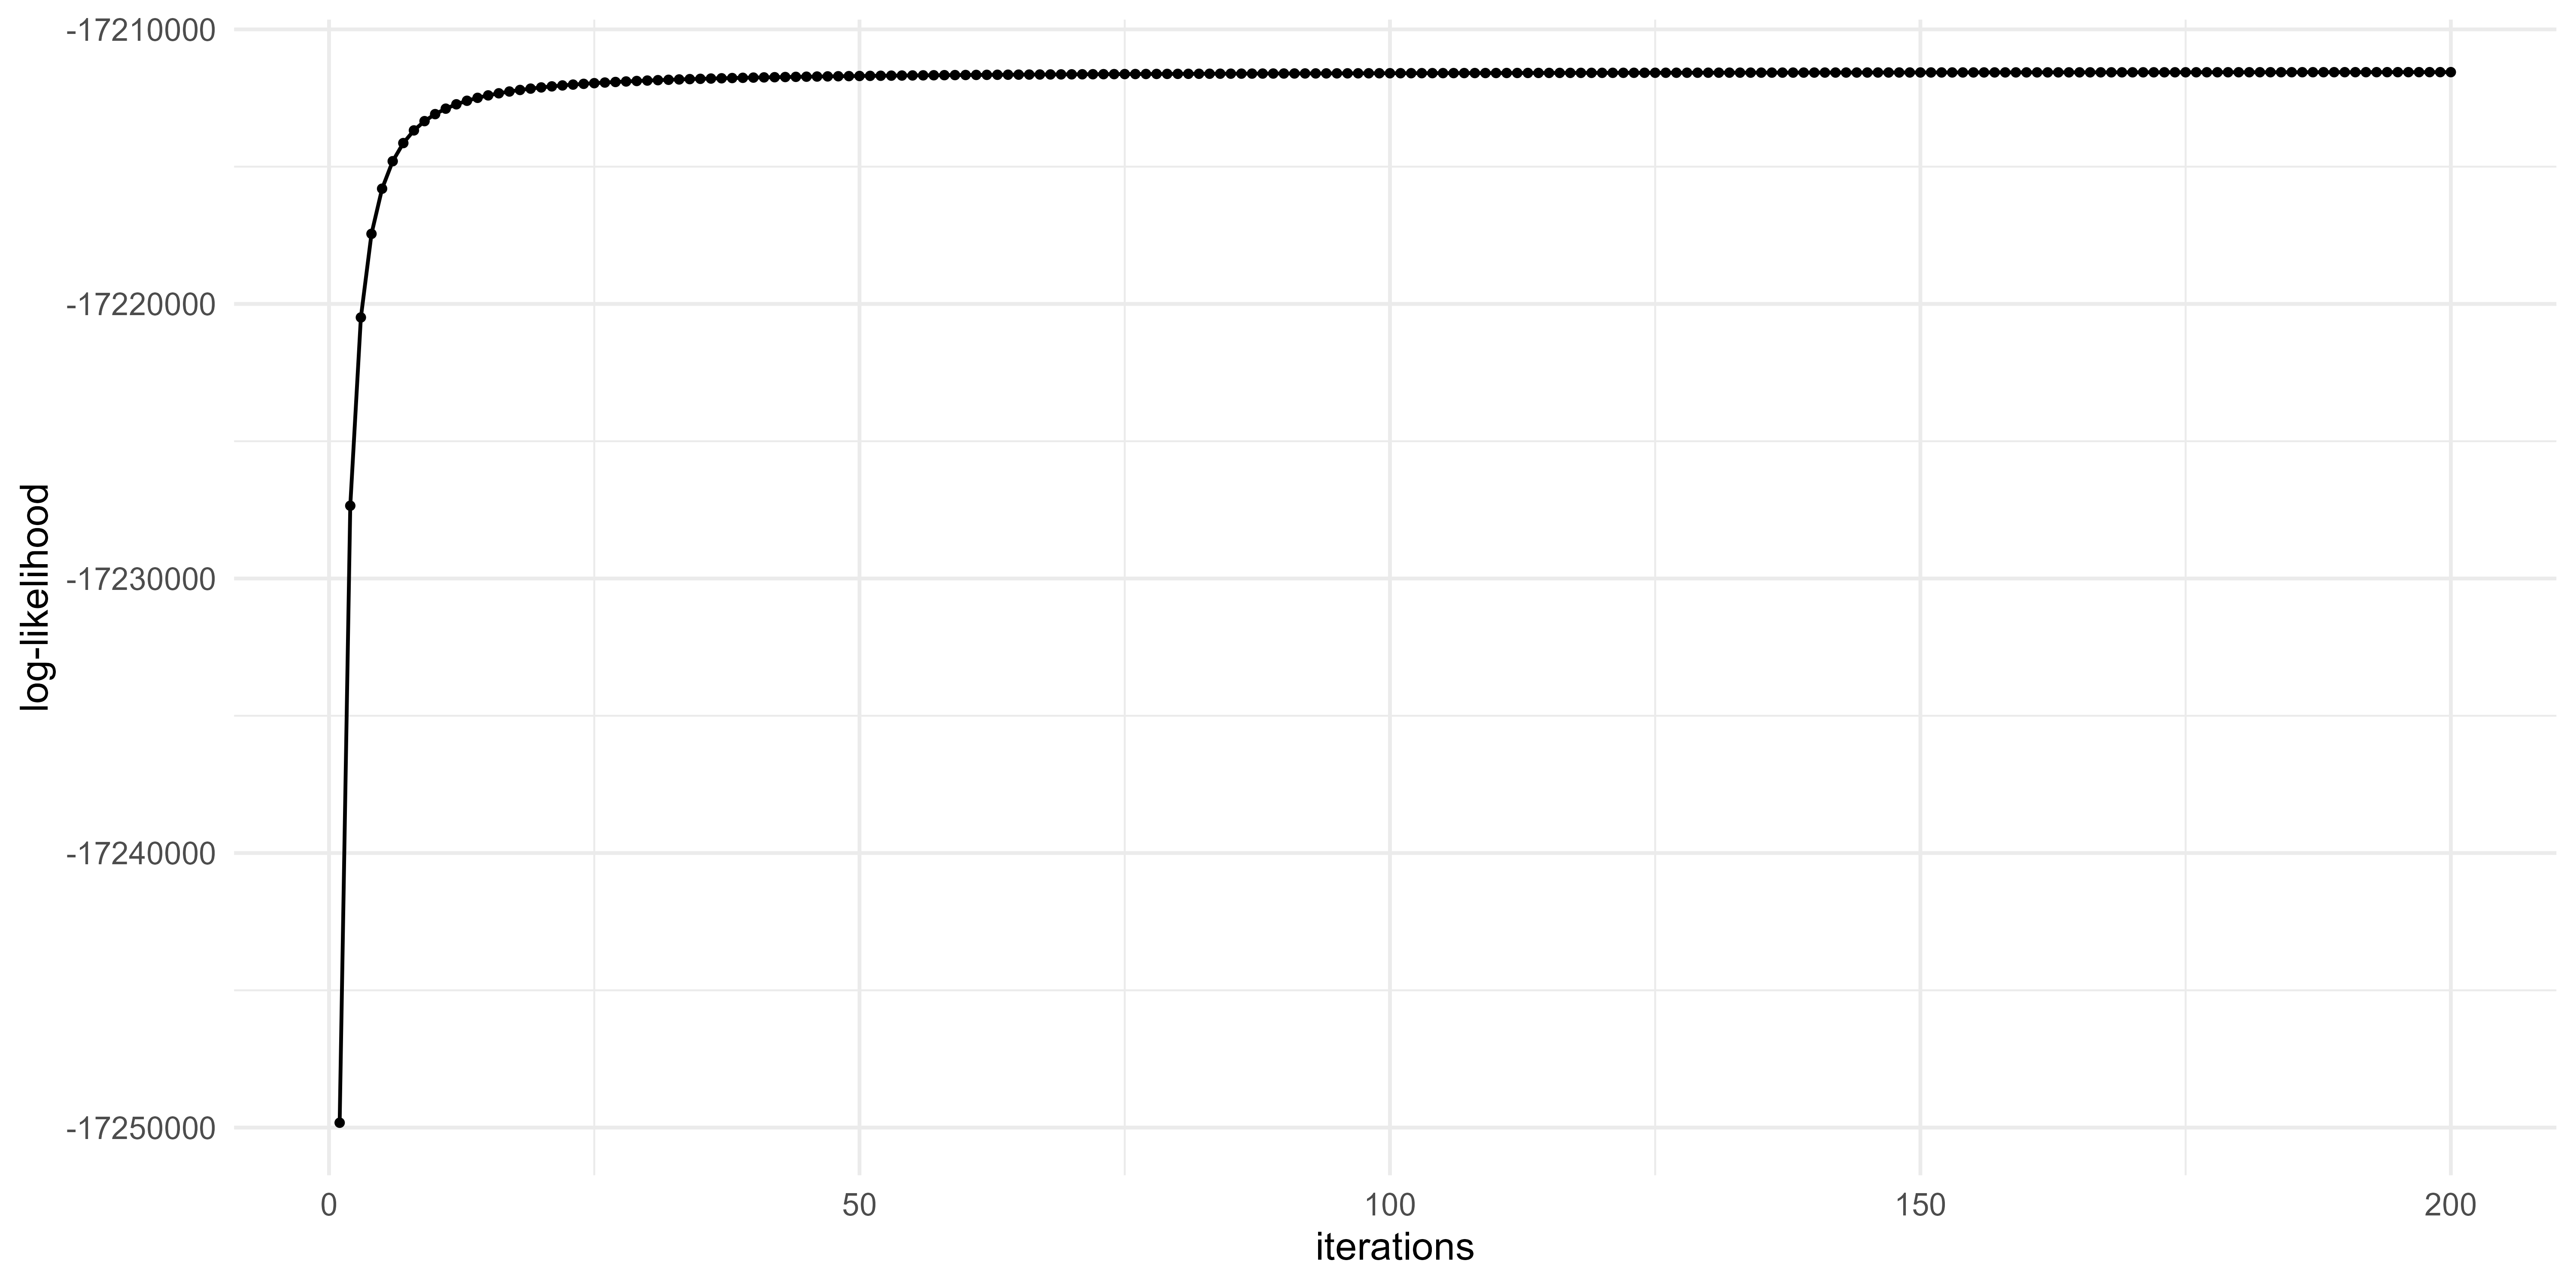
\includegraphics[width=0.5\textwidth]{figures/ll.png}
    \caption[Log-likelihood against EM iterations]{Log-likelihood against EM iterations}
    \label{fig:ll}
\end{figure}

Our EM algorithm converges quickly, with the log-likelihood non-decreasing.

\chapter{Evaluation metrics}\label{ap:eval-metrics}

In this appendix, we describe evaluation metrics used for model evaluation. Let $\bm\theta$ be the reference and $\hat{\bm\theta}$ be the estimates. 

The \textbf{Spearman correlation coefficient} (SCC) is a reference-based metric that measures the strength of monotonic relationships between the reference and estimate. Let $\bm R$ be the ranks for $\bm\theta$ and $\hat{\bm R}$ be the ranks for $\hat{\bm\theta}$. The SCC is given by
\begin{equation}
    SCC = \frac{\textrm{cov}(\bm{R},\hat{\bm{R}})}{\textrm{sd}(\bm{R})\cdot \textrm{sd}(\hat{\bm{R}})}
\end{equation}
The \textbf{relative difference} (RD) is a reference-based metric that measures relative difference of an estimate against the reference. The RD is given by
\begin{equation}
    RD = \frac{\mid\bm\theta-\hat{\bm\theta}\mid}{\bm\theta}
\end{equation}
The \textbf{normalized root-mean-squared error} (NRMSE) is a reference-based metric that measures the deviation from a linear relationship between the estimate and the reference. The NRMSE is given by
\begin{equation}
    NRMSE = \frac{\sqrt{\frac{1}{M}\sum\left(\bm\theta-\hat{\bm\theta}\right)^2}}{\textrm{sd}\left(\hat{\bm\theta}\right)}
\end{equation}
The \textbf{reproducibility metric} (RM) is a reference-free metric that measures the variance across replicates. Let $\bar{\bm\theta}$ be the mean of estimates across $K$ replicates. For isoform $j$, the RM is given by
\begin{equation}
    RM = \sqrt{\frac{1}{K}\sum_k \left(\hat{\theta_i} - \bar{\theta_i}\right)^2}
\end{equation}

\chapter{Data and code availability}

\paragraph{Data}
We used long-read RNA-seq data from the SG-NEx project available at \url{https://github.com/GoekeLab/sg-nex-data}. All simulated datasets were generated with the software below. 

\paragraph{Code}
All software was developed in \texttt{python3}. Software for generating novel isoform models and simulating degraded reads are available at \url{https://github.com/jleechung/noviso} and \url{https://github.com/jleechung/shamread} respectively. These are not implemented as CLI tools but use a yaml file for configuring inputs. Software for our quantification model is available at \url{https://github.com/jleechung/daiso} and is implemented as a CLI tool with simple installation (via conda) and user interface, with only one required input. We display the manual page here for reference: 

\VerbatimInput{figures/man.txt}